\begin{frame}
	%\frametitle{$\qquad \qquad \qquad M^{(a/b)}(t,t_s,w_\star,L) 
	%			\approx L^{-y_l} {\cal M}_i(\Upsilon,\Theta, \Theta_\star)$}
	\frametitle{First Order Quantum transition (FOQT)}

    \begin{equation}
        \label{eq:model}
        \hat{H}(h_\perp,h_\parallel)=-J\sum_{j=1}^{L-1} \hat\sigma^{(3)}_j\hat\sigma^{(3)}_{j+1} -\sum_{j=1}^L (h_\perp\hat\sigma^{(1)}_j + h_\parallel \hat\sigma^{(3)}_j).   
    \end{equation}
        
    \begin{center}
		\begin{figure}
					   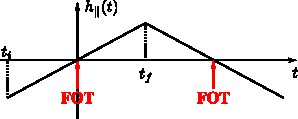
\includegraphics[width=8.4cm]{paper/protocol_foqt.pdf}
					  \caption{ FOQT Round-trip Protocol where we keep $h_\perp$ fixed and $h_\parallel (t) = t / t_s$.}
					\label{protocol_foqt}
		\end{figure}
	\end{center}
	
	
	
\end{frame}

\begin{frame}
    \frametitle{Out-Of-Equilibrium FSS at FOQT }

    Degeneracy of the 2 lowest energy level for finite $L$ approaching the FOQT point $\longrightarrow$ Two-levels model\\
    $ $\\

    We formulate the OFSS regime as the limit $L \to \infty$, $u = t_s L^{-1} M_0^{-1} \to \infty$.\\
    $ $\\
    The time-dependent expectation values of local observables are proportional to quasi-universal OFSS functions of the variables:
    \begin{align}
        \tau &= \frac{t}{\sqrt{u}} \,\,,\\
        \upsilon &= u \,\,\Delta^2(h_\perp, L) \,\,. 
    \end{align}

\end{frame}

\begin{frame}
    \frametitle{Validity of our scaling hypothesis}




    %\begin{align}
	%	M(t,t_s,w_i,L) \approx L^{-y_l} {\cal M}_i(\Upsilon,\Theta)\,\,.
	%\end{align}
	\begin{columns}
        \begin{column}{0.52\textwidth}
            \begin{figure}[t]
                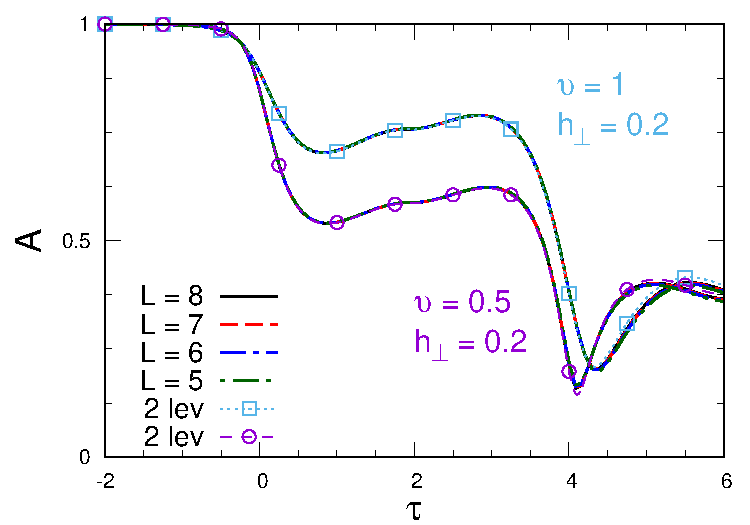
\includegraphics[width=1.\columnwidth]{paper/tripAt2u05g02-new.pdf}
                \caption{OFSS  of the adiabaticity function in $A(h_\perp,t,t_s,L)\sim {\cal F}_A(\tau,\upsilon)$ shown as a function of the rescaled time $\tau$ during a round-trip protocol with $|\tau_i|=\tau_f =2$ (FOTs at $\tau=0,4$).}
                \label{AtripAt2u05g02}
            \end{figure}
        \end{column}
        \begin{column}{0.5\textwidth}
            \begin{figure}[t]
                \centering
                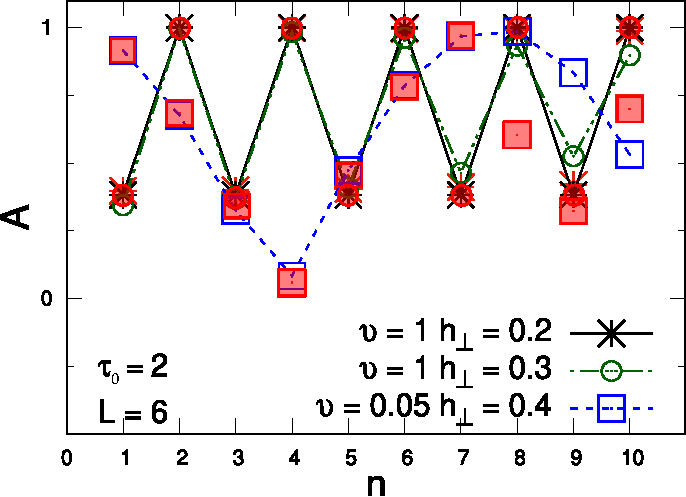
\includegraphics[width=1.\columnwidth]{paper/strobA.pdf}
                \caption{Stroboscopic evolution of $A$  as function of  $n$ (corresponding to times $t=t_0(4n-1)$) at fixed $L=6$, $\tau_0=2$}\label{fig:strobo}
            \end{figure}
        \end{column}
        \end{columns}
\end{frame}


\begin{frame}
    \frametitle{ Effective description in the OFSS regime}

    Emergence of an effective two-level description which involves the lowest two states near the FOT. \\
    $ $\\
    With this effective description, we reduce the driving protocol to a series of LZS and we determine an analytical expression of the OFSS functions:
    \begin{align}
        {\cal F}_A(\tau,\upsilon)
        \nonumber
        &=e^{-\frac{\pi\upsilon}{32}}\Bigg|\sqrt{\frac{1}{2}+ \frac{|\tau|}{\sqrt{4\tau^2+\upsilon}}} \mathscr{D}_{\frac{i u}{8}}(\sqrt{2}e^{i\frac{3\pi}{4}}\tau) 
        \nonumber\\
        &\quad -\frac{\sqrt{\upsilon} e^{-\frac{i\pi}{4}}}{2\sqrt{2}} \sqrt{\frac{1}{2}- \frac{|\tau|}{\sqrt{4\tau^2+\upsilon}}} \mathscr{D}_{-1+\frac{i u}{8}}(\sqrt{2}e^{i\frac{3\pi}{4}}\tau)\Bigg|
    \end{align}

    $ $\\
    {\bf Breakdown of the effective description}\\

    Corrections to the scaling behavior are expected when:
    \begin{align}
        \tau   \gtrsim O(t_{KZ}) 
        \qquad {\rm with} \qquad
        t_{KZ} & = \sqrt{u} \,\,.
    \end{align}

\end{frame}